\chapter{Some topological constructions}
In this short chapter we briefly describe some common spaces and constructions
in topology that we haven't yet discussed.

\section{Spheres}
Recall that
\[ S^n = \left\{ (x_0, \dots, x_n)
	\mid x_0^2 + \dots + x_n^2 = 1 \right\} \subset \RR^{n+1} \]
is the surface of an $n$-sphere while
\[ D^{n+1} = \left\{ (x_0, \dots, x_n)
	\mid x_0^2 + \dots + x_n^2 \le 1 \right\} \subset \RR^{n+1} \]
is the corresponding \emph{closed disk}
(So for example, $D^2$ is a disk in a plane while $S^1$ is the unit circle.)
\begin{exercise}
	Show that the open disk $D^n \setminus S^{n-1}$
	is homeomorphic to $\RR^n$.
\end{exercise}

In particular, $S^0$ consists of two points,
while $D^1$ can be thought of as the interval $[-1,1]$.

\begin{center}
	\begin{asy}
		size(8cm);
		draw(dir(0)--dir(180), blue);
		dot(dir(0), red+4);
		dot(dir(180), red+4);
		label("$S^0$", dir(0), dir(90), red);
		label("$D^1$", dir(0)--dir(180), blue);
		add(shift(-4,0)*CC());
		unitsize(2cm);
		filldraw(unitcircle, lightblue+opacity(0.2), red);
		label("$D^2$", origin, blue);
		label("$S^1$", dir(45), dir(45), red);
	\end{asy}
\end{center}


\section{Quotient topology}
\prototype{$D^n / S^{n-1} = S^n$, or the torus.}

Given a space $X$, we can \emph{identify} some of the points together
by any equivalence relation $\sim$;
for an $x \in X$ we denote its equivalence class by $[x]$.
Geometrically, this is the space achieved by welding together points
equivalent under $\sim$.

Formally,
\begin{definition}
	Let $X$ be a topological space, and $\sim$ an equivalence relation
	and the points of $X$.
	Then $X / {\sim}$ is the space whose
	\begin{itemize}
		\ii Points are equivalence classes of $X$, and
		\ii $U \subseteq X / {\sim}$ is open if and only if
		$\left\{ x \in X \text{ such that } [x] \in U  \right\}$
		is open in $X$.
	\end{itemize}
\end{definition}
As far as I can tell, this definition is mostly useless for intuition,
so here are some examples.

\begin{example}[Interval modulo endpoints]
	Suppose we take $D^1 = [-1, 1]$
	and quotient by the equivalence relation which identifies
	the endpoints $-1$ and $1$.
	(Formally, $x \sim y \iff (x=y) \text{ or } \{x,y\} = \{-1,1\}$.)
	In that case, we simply recover $S^1$:
	\begin{center}
		\begin{asy}
			size(8cm);
			draw(dir(0)--dir(180), blue);
			dot("$-1$", dir(0), dir(90), red+4);
			dot("$-1$", dir(180), dir(90), red+4);
			label("$D^1$", dir(0)--dir(180), blue);
			add(shift(-4,0)*CC());
			unitsize(2cm);
			draw(unitcircle, blue);
			label("$S^1 \approx D^1 / {\sim}$", dir(45), dir(45), blue);
			dot("$-1 \sim 1$", dir(90), dir(90), red);
		\end{asy}
	\end{center}
	Observe that a small neighborhood around $-1 \sim 1$ in the quotient space
	corresponds to two half-intervals at $-1$ and $1$ in the original space $D^1$.
	This should convince you the definition we gave is the right one.
\end{example}

\begin{example}[More quotient spaces]
	Convince yourself each of the following is correct:
	\begin{itemize}
		\ii Generalizing the previous example, $D^n$ modulo its boundary $S^{n-1}$ is $S^n$.
		\ii Given a square $ABCD$, suppose we identify segments $AB$ and $DC$ together.
		Then we get a cylinder. (Think elementary school, when you would tape
		up pieces of paper together to get cylinders.)
		\ii In the previous example, if we also identify $BC$ and $DA$ together,
		then we get a torus. (Imagine taking our cylinder and putting the two
		circles at the end together.)
		\ii Let $X = \RR$, and let $x \sim y$ if $y -x \in \ZZ$.
		Then $X / {\sim}$ is $S^1$ as well.
	\end{itemize}
\end{example}

One special case that we did above:
\begin{definition}
	Let $A \subseteq X$.
	Consider the equivalence relation which identifies
	all the points of $A$ with each other
	while leaving all remaining points inequivalent.
	(In other words, $x \sim y$ if $x=y$ or $x,y \in A$.)
	Then the resulting quotient space is denoted $X/A$.
\end{definition}

So in this notation, \[ D^n / S^{n-1} = S^n. \]

\begin{abuse}
	Note that I'm deliberately being sloppy, and saying
	``$D^n / S^{n-1} = S^n$'' or ``$D^n / S^{n-1}$ \emph{is} $S^n$'',
	when I really ought to say ``$D^n / S^{n-1}$ is homeomorphic to $S^n$''.
	This is a general theme in mathematics:
	objects which are homoeomorphic/isomorphic/etc.\ are generally
	not carefully distinguished from each other.
\end{abuse}

\section{Product topology}
\prototype{$\RR \times \RR$ is $\RR^2$, $S^1 \times S^1$ is the torus.}

\begin{definition}
	Given topological spaces $X$ and $Y$,
	the product space $X \times Y$ is the space whose
	\begin{itemize}
		\ii Points are pairs $(x,y)$ with $x \in X$, $y \in Y$, and
		\ii Topology is given as follows: the \emph{basis} of
		the topology for $X \times Y$ is $U \times V$,
		for $U \subseteq X$ open and $V \subseteq Y$ open.
	\end{itemize}
\end{definition}
\begin{remark}
	It is not hard to show that, in fact,
	one need only consider basis elements for $U$ and $V$.
	That is to say,
	\[ \left\{ U \times V \mid
		U,V \text{ basis elements for } X,Y \right\} \]
	is also a basis for $X \times Y$.
\end{remark}

This does exactly what you think it would.
\begin{example}[The unit square]
	Let $X = [0,1]$ and consider $X \times X$.
	We of course expect this to be the unit square.
	Pictured below is an open set of $X \times X$ in the basis.
	\begin{center}
		\begin{asy}
		size(6cm);
		filldraw(unitsquare, opacity(0.2)+lightblue, black);

		pair B = (0,1);
		pair A = (1,0);
		fill(box(0.3*A+0.2*B,0.6*A+0.7*B), lightred+opacity(0.5));
		label("$U \times V$", (0.45,0.45), brown);

		draw(0.3*A--(0.3*A+B), heavygreen+dashed+1);
		draw(0.6*A--(0.6*A+B), heavygreen+dashed+1);
		draw(0.2*B--(0.2*B+A), heavycyan+dashed+1);
		draw(0.7*B--(0.7*B+A), heavycyan+dashed+1);

		draw( 0.3*A--0.6*A, heavygreen+2 );
		opendot( 0.3*A,  heavygreen+2);
		opendot( 0.6*A, heavygreen+2);
		label("$U$", 0.45*A, dir(-90), heavygreen);
		draw( 0.2*B--0.7*B, heavycyan+2 );
		opendot( 0.2*B, heavycyan+2);
		opendot( 0.7*B, heavycyan+2);
		label("$V$", 0.45*B, dir(180), heavycyan);
		\end{asy}
	\end{center}
\end{example}
\begin{exercise}
	Convince yourself this basis gives the same topology
	as the product metric on $X \times X$.
	So this is the ``right'' definition.
\end{exercise}

\begin{example}[More product spaces]
	\listhack
	\begin{enumerate}[(a)]
		\ii $\RR \times \RR$ is the Euclidean plane.
		\ii $S^1 \times [0,1]$ is a cylinder.
		\ii $S^1 \times S^1$ is a torus! (Why?)
	\end{enumerate}
\end{example}

\section{Disjoint union and wedge sum}
\prototype{$S^1 \wedge S^1$ is the figure eight.}

The disjoint union of two spaces is geometrically exactly
what it sounds like: you just imagine the two spaces side by side.
For completeness, here is the formal definition.
\begin{definition}
	Let $X$ and $Y$ be two topological spaces.
	The \vocab{disjoint union}, denoted $X \amalg Y$, is defined by
	\begin{itemize}
		\ii The points are the disjoint union $X \sqcup Y$, and
		\ii A subset $U \subseteq X \sqcup Y$ is open if
		and only if $U \cap X$ and $U \cap Y$ are open.
	\end{itemize}
\end{definition}
\begin{exercise}
	Show that the disjoint union of two nonempty spaces is disconnected.
\end{exercise}

More interesting is the wedge sum, where two topological spaces $X$
and $Y$ are fused together only at a single base point.
\begin{definition}
	Let $X$ and $Y$ be topological spaces, and $x_0 \in X$ and $y_0 \in Y$
	be points.
	We define the equivalence relation $\sim$ by declaring $x_0 \sim y_0$ only.
	Then the \vocab{wedge sum} of two spaces is defined as
	\[ X \vee Y = (X \amalg Y) / {\sim}. \]
\end{definition}

\begin{example}
	[$S^1 \vee S^1$ is a figure eight]
	Let $X = S^1$ and $Y = S^1$,
	and let $x_0 \in X$ and $y_0 \in Y$ be any points.
	Then $X \vee Y$ is a ``figure eight'': it is two
	circles fused together at one point.
	\begin{center}
		\begin{asy}
			size(3cm);
			draw(shift(-1,0)*unitcircle);
			draw(shift(1,0)*unitcircle);
			dotfactor *= 1.4;
			dot(origin);
		\end{asy}
	\end{center}
\end{example}
\begin{abuse}
	We often don't mention $x_0$ and $y_0$ when they are understood
	(or irrelevant).  For example, from now on we will just
	write $S^1 \vee S^1$ for a figure eight.
\end{abuse}

\begin{remark}
	Annoyingly, in \LaTeX\ \verb+\wedge+ gives $\wedge$ instead
	of $\vee$ (which is \verb+\vee+).
	So this really should be called the ``vee product'', but too late.
\end{remark}


\section{CW complexes}
Using this construction, we can start building some spaces.
One common way to do so is using a so-called \vocab{CW complex}.
Intuitively, a CW complex is built as follows:
\begin{itemize}
	\ii Start with a set of points $X^0$.
	\ii Define $X^1$ by taking some line segments (copies of $D^1$)
	and fusing the endpoints (copies of $S^0$) onto $X^0$.
	\ii Define $X^2$ by taking copies of $D^2$ (a disk)
	and welding its boundary (a copy of $S^1$) onto $X^1$.
	\ii Repeat inductively up until a finite stage $n$;
	we say $X$ is \vocab{$n$-dimensional}.
\end{itemize}
The resulting space $X$ is the CW-complex.
The set $X^k$ is called the \vocab{$k$-skeleton} of $X$.
Each $D^k$ is called a \vocab{$k$-cell}; it is customary to
denote it by $e_\alpha^k$ where $\alpha$ is some index.
We say that $X$ is \vocab{finite} if only finitely many cells were used.
\begin{abuse}
	Technically, most sources (like \cite{ref:hatcher}) allow one to
	construct infinite-dimensional CW complexes.
	We will not encounter any such spaces in the Napkin.
\end{abuse}

\begin{example}
	[$D^2$ with $2+2+1$ and $1+1+1$ cells]
	\listhack
	\begin{enumerate}[(a)]
	\ii First, we start with $X^0$ having two points $e_a^0$ and $e_b^0$.
	Then, we join them with two $1$-cells $D^1$ (green),
	call them $e_c^1$ and $e_d^1$.
	The endpoints of each $1$-cell (the copy of $S^0$) get identified
	with distinct points of $X^0$; hence $X^1 \cong S^1$.
	Finally, we take a single $2$-cell $e^2$ (yellow) and weld it in,
	with its boundary fitting into the copy of $S^1$ that we just drew.
	This gives the figure on the left.

	\ii In fact, one can do this using just $1+1+1=3$ cells.
	Start with $X^0$ having a single point $e^0$.
	Then, use a single $1$-cell $e^1$, fusing its two endpoints
	into the single point of $X^0$.
	Then, one can fit in a copy of $S^1$ as before,
	giving $D^2$ as on the right.
	\end{enumerate}
	\begin{center}
		\begin{asy}
			size(4cm);
			filldraw(unitcircle, opacity(0.2)+yellow, heavygreen);
			dotfactor *= 1.4;
			dot(dir(90), blue);
			dot(dir(-90), blue);
			label("$e_a^0$", dir(90), dir(90), blue);
			label("$e_b^0$", dir(-90), dir(-90), blue);
			label("$e_c^1$", dir(0), dir(0), heavygreen);
			label("$e_d^1$", dir(180), dir(180), heavygreen);
			label("$e^2$", origin, origin);
		\end{asy}
		\qquad
		\begin{asy}
			size(4cm);
			filldraw(unitcircle, opacity(0.2)+yellow, heavygreen);
			dotfactor *= 1.4;
			dot(dir(90), blue);
			label("$e^0$", dir(90), dir(90), blue);
			label("$e^1$", dir(-90), dir(-90), heavygreen);
			label("$e^2$", origin, origin);
		\end{asy}
	\end{center}
\end{example}

\begin{example}
	[$S^n$ as a cW complex]
	\listhack
	\begin{enumerate}[(a)]
		\ii One can obtain $S^n$ (for $n \ge 1$) with just two cells.
		Namely, take a single point $e^0$ for $X^0$, and to obtain $S^n$
		take $D^n$ and weld its entire boundary into $e^0$.

		We already saw this example in the beginning with $n=2$,
		when we saw that the sphere $S^2$ was the result when we fuse
		the boundary of a disk $D^2$ together.
		
		\ii Alternatively, one can do a ``hemisphere'' construction,
		by construction $S^n$ inductively using two cells in each dimension.
		So $S^0$ consists of two points, then $S^1$ is obtained
		by joining these two points by two segments ($1$-cells),
		and $S^2$ is obtained by gluing two hemispheres (each a $2$-cell)
		with $S^1$ as its equator.
	\end{enumerate}
\end{example}

\begin{definition}
	Formally, for each $k$-cell $e^k_\alpha$ we want to add to $X^k$,
	we take its boundary $S^{k-1}_\alpha$ and weld it onto
	$X^{k-1}$ via an \vocab{attaching map} $S^{k-1}_\alpha \to X^{k-1}$.
	Then
	\[ X^k = X^{k-1} \amalg \left(\coprod_\alpha e^k_\alpha\right) / {\sim} \]
	where $\sim$ identifies each boundary point of $e_k^\alpha$
	with its image in $X^{k-1}$.
\end{definition}


\section{The torus, Klein bottle, $\RP^n$, $\CP^n$}
We now present four of the most import examples of CW complexes.

\subsection*{The torus}
The \vocab{torus} can be formed by taking
a square and identifying the opposite edges in the same direction:
if you walk off the right edge, you re-appear at the corresponding
point in on the left edge.
(Think \emph{Asteroids} from Atari!)

\begin{center}
	\begin{asy}
		size(2cm);
		fill(unitsquare, yellow+opacity(0.2));
		pair C = (0,0);
		pair B = (1,0);
		pair A = (1,1);
		pair D = (0,1);
		draw(A--B, red, MidArrow);
		draw(B--C, blue, MidArrow);
		draw(D--C, red, MidArrow);
		draw(A--D, blue, MidArrow);
	\end{asy}
\end{center}

Thus the torus is $(\RR/\ZZ)^2 \cong S^1 \times S^1$.

Note that all four corners get identified together to a single point.  One
can realize the torus in $3$-space by treating the square as a sheet of paper,
taping together the left and right (red) edges to form a cylinder,
then bending the cylinder and fusing the top and bottom (blue) edges
to form the torus.
\begin{center}
	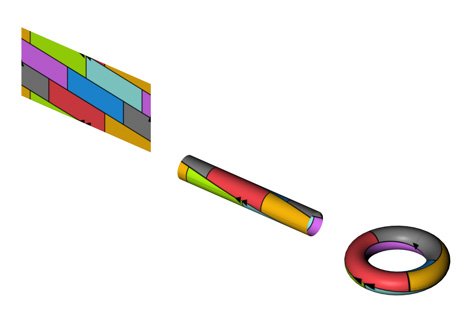
\includegraphics[width=0.8\textwidth]{media/Projection_color_torus.jpg} \\ \tiny
	\url{https://en.wikipedia.org/wiki/File:Projection_color_torus.jpg}
	(public domain)
\end{center}

The torus can be realized as a CW complex with
\begin{itemize}
	\ii A $0$-skeleton consisting of a single point,
	\ii A $1$-skeleton consisting of two $1$-cells $e^1_a$, $e^1_b$, and
	\begin{center}
		\begin{asy}
			unitsize(1cm);
			draw(shift(-1,0)*unitcircle, blue, MidArrow);
			draw(shift(1,0)*rotate(180)*unitcircle, red, MidArrow);
			label("$e^1_a$", 2*dir(180), dir(180), blue);
			label("$e^1_b$", 2*dir(0), dir(0), red);
			dotfactor *= 1.4;
			dot("$e^0$", origin, dir(0));
		\end{asy}
	\end{center}
	\ii A $2$-skeleton with a single $2$-cell $e^2$,
	whose circumference is divided into four parts,
	and welded onto the $1$-skeleton ``via $aba\inv b \inv$''.
	This means: wrap a quarter of the circumference around $e^1_a$,
	then another quarter around $e^1_b$,
	then the third quarter around $e^1_a$ but in the opposite direction,
	and the fourth quarter around $e^1_b$ again in the opposite direction as before.
	\begin{center}
		\begin{asy}
			size(3cm);
			fill(unitcircle, yellow+opacity(0.2));
			defaultpen(linewidth(1));
			draw(arc(origin, 1, 45, 135), blue, MidArrow);
			draw(arc(origin, 1, 315, 225), blue, MidArrow);
			draw(arc(origin, 1, 135, 225), red, MidArrow);
			draw(arc(origin, 1, 45, -45), red, MidArrow);
			label("$e^2$", origin, origin);
		\end{asy}
	\end{center}
\end{itemize}
We say that $aba\inv b\inv$ is the \vocab{attaching word};
this shorthand will be convenient later on.

\subsection*{The Klein bottle}
The \vocab{Klein bottle} is defined similarly to
the torus, except one pair of edges is identified in the opposite manner,
as shown.

\begin{center}
	\begin{asy}
		size(2cm);
		fill(unitsquare, yellow+opacity(0.2));
		pair C = (0,0);
		pair B = (1,0);
		pair A = (1,1);
		pair D = (0,1);
		draw(A--B, red, MidArrow);
		draw(C--B, blue, MidArrow);
		draw(D--C, red, MidArrow);
		draw(A--D, blue, MidArrow);
	\end{asy}
\end{center}

Unlike the torus one cannot realize this in $3$-space
without self-intersecting. One can tape together the red edges
as before to get a cylinder, but to then fuse the resulting blue
circles in opposite directions is not possible in 3D.
Nevertheless, we often draw a picture in 3-dimensional space
in which we tacitly allow the cylinder to intersect itself.

\begin{center}
	\begin{minipage}[c]{0.5\textwidth}
	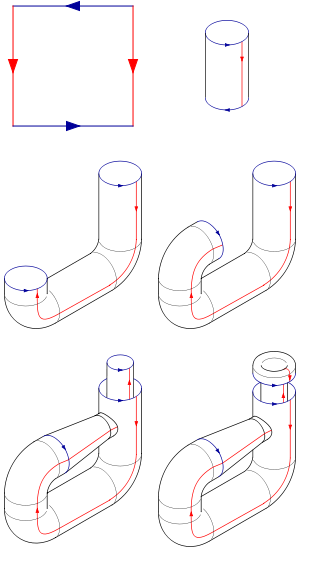
\includegraphics[width=\textwidth]{media/klein-fold.png}
	\end{minipage}
	\quad
	\begin{minipage}[c]{0.3\textwidth}
	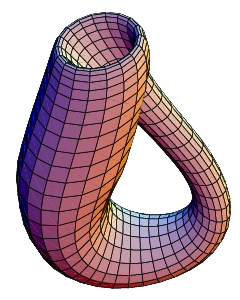
\includegraphics[width=\textwidth]{media/KleinBottle-01.png}
	\end{minipage}

	\tiny
	\url{https://commons.wikimedia.org/wiki/File:Klein_Bottle_Folding_1.svg} \\
	\url{https://en.wikipedia.org/wiki/File:KleinBottle-01.png} \\
	(public domain)
\end{center}


Like the torus, the Klein bottle is realized as a CW complex with
\begin{itemize}
	\ii One $0$-cell,
	\ii Two $1$-cells $e^1_a$ and $e^1_b$, and
	\ii A single $2$-cell attached this time via the word $abab\inv$.
\end{itemize}

\subsection*{Real projective space}
Let's start with $n=2$.
The space $\RP^2$ is obtained if we reverse both directions of
the square from before, as shown.

\begin{center}
	\begin{asy}
		size(2cm);
		fill(unitsquare, yellow+opacity(0.2));
		pair C = (0,0);
		pair B = (1,0);
		pair A = (1,1);
		pair D = (0,1);
		draw(B--A, red, MidArrow);
		draw(C--B, blue, MidArrow);
		draw(D--C, red, MidArrow);
		draw(A--D, blue, MidArrow);
	\end{asy}
\end{center}

However, once we do this the fact that the original
polygon is a square is kind of irrelevant;
we can combine a red and blue edge to get the single purple edge.
Equivalently, one can think of this as a circle with half
its circumference identified with the other half:

\begin{center}
	\begin{asy}
		size(3cm);
		dotfactor *= 2;
		fill(unitcircle, opacity(0.2)+yellow);
		draw(dir(-90)..dir(0)..dir(90), purple, MidArrow);
		draw(dir(90)..dir(180)..dir(-90), purple, MidArrow);
		dot(dir(90));
		dot(dir(-90));
		label("$\mathbb{RP}^2$", origin, origin);
	\end{asy}
	\qquad
	\begin{asy}
		size(3cm);
		dotfactor *= 2;
		draw(dir(-90)..dir(0)..dir(90));
		draw(dir(90)..dir(180)..dir(-90), dashed);
		fill(unitcircle, yellow+opacity(0.2));
		dot(dir(90));
		opendot(dir(-90));
		label("$\mathbb{RP}^2$", origin, origin);
	\end{asy}
\end{center}

The resulting space should be familiar to those of you who do
projective (Euclidean) geometry.
Indeed, there are several possible geometric interpretations:
\begin{itemize}
	\ii One can think of $\RP^2$ as the set of lines through the
	origin in $\RR^3$, with each line being a point in $\RP^2$.

	Of course, we can identify each line with a point on the unit sphere $S^2$,
	except for the property that two antipodal points actually 
	correspond to the same line, so that $\RP^2$ can be almost thought
	of as ``half a sphere''. Flattening it gives the picture above.

	\ii Imagine $\RR^2$, except augmented with ``points at infinity''.
	This means that we add some lines ``infinitely far away'',
	one for each possible direction of a line.
	Thus in $\RP^2$, any two lines indeed intersect
	(at a Euclidean point if they are not parallel, and at a line
	at infinity if they do).

	This gives an interpretation of $\RP^2$,
	where the boundary represents the \emph{line at infinity}
	through all of the points at infinity.
	Here we have used the fact that $\RR^2$
	and interior of $D^2$ are homeomorphic.
\end{itemize}
\begin{exercise}
	Observe that these formulations are equivalent
	by consider the plane $z=1$ in $\RR^3$,
	and intersecting each line in the first formulation with this plane.
\end{exercise}

We can also express $\RP^2$ using coordinates:
it is the set of triples $(x : y : z)$ of real numbers not all zero
up to scaling, meaning that 
\[ (x : y : z) = (\lambda x : \lambda y : \lambda z) \]
for any $\lambda \neq 0$.
Using the ``lines through the origin in $\RR^3$'' interpretation
makes it clear why this coordinate system gives the right space.
The points at infinity are those with $z = 0$,
and any point with $z \neq 0$ gives a Cartesian point since
\[ (x : y : z) = \left( \frac xz : \frac yz : 1 \right) \]
hence we can think of it as the Cartesian point $(\frac xz, \frac yz)$.

In this way we can actually define \vocab{real-projective $n$-space},
$\RP^n$ for any $n$, as either
\begin{enumerate}[(i)]
	\ii The set of lines through the origin in $\RR^{n+1}$,
	\ii Using $n+1$ coordinates as above, or
	\ii As $\RR^n$ augmented with points at infinity,
	which themselves form a copy of $\RP^{n-1}$.
\end{enumerate}

As a possibly helpful example, we draw all three pictures of $\RP^1$.
\begin{example}
	[Real projective $1$-Space]
	$\RP^1$ can be thought of as $S^1$ modulo the relation
	the antipodal points are identified.
	Projecting onto a tangent line, we see that we get
	a copy of $\RR$ plus a single point at infinity, corresponding
	to the parallel line (drawn in cyan below).
	\begin{center}
		\begin{asy}
			size(8cm);
			filldraw(unitcircle, lightblue+opacity(0.2), heavyblue+opacity(0.4));
			label("$S^1$", dir(225), dir(225), lightblue);
			dot("$\vec 0$", origin, dir(45));
			pair X1 = (-2.1,1);
			pair X2 = (1.9,1);
			draw(X1--X2, heavyred, Arrows);
			dot("$0$", (0,1), dir(90), heavyred);
			dot("$1$", (1,1), dir(90), heavyred);
			pair P = extension( (0,1), (1,1), dir(250), dir(70) );
			dot("$0.36$", P, dir(90), heavyred);
			label("$\mathbb R$", X2, dir(105), heavyred);
			draw(L(dir(130),-dir(130),0.2,0.2), gray);
			draw(L(dir(250),-dir(250),0.2,0.2), gray);
			draw(L(dir(-20),-dir(-20),0.2,0.2), gray);
			draw(L(dir(0), -dir(0), 0.4,0.4), heavycyan+1);
		\end{asy}
	\end{center}
	Thus, the points of $\RP^1$ have two forms:
	\begin{itemize}
		\ii $(x:1)$, which we think of as $x \in \RR$ (in dark red above), and
		\ii $(1:0)$, which we think of as $1/0 = \infty$,
		corresponding to the cyan line above.
	\end{itemize}
	So, we can literally write
	\[ \RP^1 = \RR \cup \{\infty\}. \]
	Note that $\RP^1$ is also the boundary of $\RP^2$.
	In fact, note also that topologically we have
	\[ \RP^1 \cong S^1 \]
	since it is the ``real line with endpoints fused together''.
	\begin{center}
		\begin{asy}
			size(2cm);
			draw(unitcircle, heavyred);
			dot("$\infty$", dir(90), dir(90), heavycyan);
			dot("$0$", dir(-90), dir(-90), heavyred);
		\end{asy}
	\end{center}
\end{example}

Since $\RP^n$ is just ``$\RR^n$ (or $D^n$) with $\RP^{n-1}$ as its boundary'',
we can construct $\RP^n$ as a CW complex inductively,
with exactly one cell in each dimension.
Thus
\begin{moral}
	$\RP^n$ consists of one cell in each dimension.
\end{moral}
For example, in low dimensions:
\begin{example}[$\RP^n$ as a cell complex]
	\listhack
	\begin{enumerate}[(a)]
		\ii $\RP^0$ is a single point.
		\ii $\RP^1 \cong S^1$ is a circle, which as a CW complex
		is a $0$-cell plus a $1$-cell.
		\ii $\RP^2$ can be formed by taking a $2$-cell
		and wrapping its perimeter twice around a copy of $\RP^1$.
	\end{enumerate}
\end{example}

\subsection*{Complex projective space}
The \vocab{complex projective space} $\CP^n$ is
defined like $\RP^n$ with coordinates, i.e.\
\[ (z_0 : z_1 : \dots : z_n) \]
under scaling.
The difference is that, as the name suggests, the coordinates
are complex numbers rather than real numbers.

As before, $\CP^n$ can be thought of as $\CC^n$ augmented
with some points at infinity (corresponding to $\CP^{n-1}$).
\begin{example}
	[Complex projective space]
	\listhack
	\begin{enumerate}[(a)]
		\ii $\CP^0$ is a single point.
		\ii $\CP^1$ is $\CC$ plus a single point at infinity
		(``complex infinity'' if you will).
		That means as before we can think of $\CP^1$ as
		\[ \CP^1 = \CC \cup \{\infty\}. \]
		So, imagine taking the complex plane and then adding
		a single point to encompass the entire boundary.
		The result is just sphere $S^2$.
	\end{enumerate}
	Here is a picture of $\CP^1$ with its coordinate system,
	idealized as the \vocab{Riemann sphere}.
	\begin{center}
		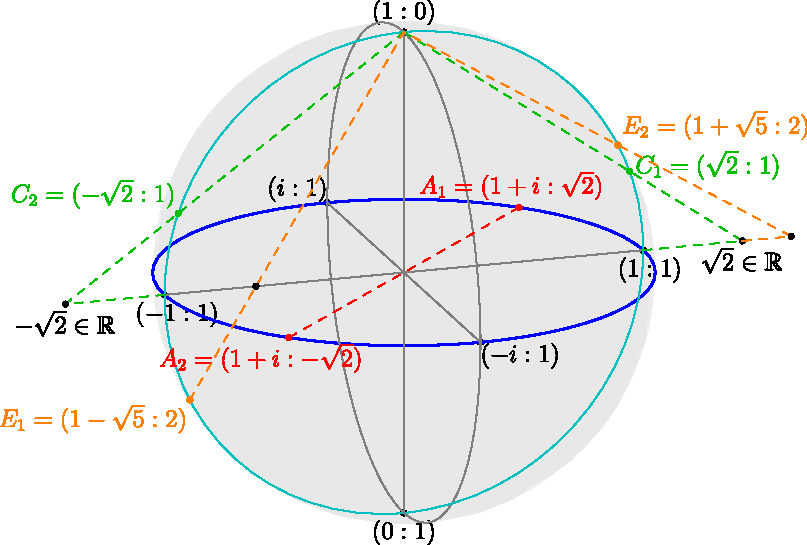
\includegraphics[width=0.9\textwidth]{media/earth.pdf}
	\end{center}
\end{example}

\begin{remark}
	[For Euclidean geometers]
	You may recognize that while $\RP^2$ is the setting for projective geometry,
	inversion about a circle is done in $\CP^1$ instead.
	When one does an inversion sending generalized circles to generalized
	circles, there is only one point at infinity:
	this is why we work in $\CP^n$.
\end{remark}

Like $\RP^n$, $\CP^n$ is a CW complex, built inductively
by taking $\CC^n$ and welding its boundary onto $\CP^{n-1}$
The difference is that as topological spaces,
\[ \CC^n \cong \RR^{2n} \cong D^{2n}. \]
Thus, we attach the cells $D^0$, $D^2$, $D^4$ and so on
inductively to construct $\CP^n$.
Thus we see that
\begin{moral}
	$\CP^n$ consists of one cell in each \emph{even} dimension.
\end{moral}


\section\problemhead
\begin{problem}
	Show that a space $X$ is Hausdorff if and only if the diagonal
	$\{(x,x) \mid x \in X\}$ is closed in the product space $X \times X$.
\end{problem}
\begin{problem}
	Realize the following spaces as a CW complex:
	\begin{enumerate}[(a)]
		\ii M\"obius strip.
		\ii $\RR$.
		\ii $\RR^n$.
	\end{enumerate}
\end{problem}
\begin{dproblem}
	Show that a finite CW complex is compact.
	\begin{hint}
		Prove and use the fact that a quotients of compact spaces remain compact.
	\end{hint}
\end{dproblem}
